
%%%%%%%%%%%%%%%%%%%%%%% file typeinst.tex %%%%%%%%%%%%%%%%%%%%%%%%%
%
% This is the LaTeX source for the instructions to authors using
% the LaTeX document class 'llncs.cls' for contributions to
% the Lecture Notes in Computer Sciences series.
% http://www.springer.com/lncs       Springer Heidelberg 2006/05/04
%
% It may be used as a template for your own input - copy it
% to a new file with a new name and use it as the basis
% for your article.
%
% NB: the document class 'llncs' has its own and detailed documentation, see
% ftp://ftp.springer.de/data/pubftp/pub/tex/latex/llncs/latex2e/llncsdoc.pdf
%
%%%%%%%%%%%%%%%%%%%%%%%%%%%%%%%%%%%%%%%%%%%%%%%%%%%%%%%%%%%%%%%%%%%


\documentclass[runningheads,a4paper]{llncs}

\usepackage{amssymb}
\setcounter{tocdepth}{3}
\usepackage{graphicx}
\usepackage{graphicx}
\usepackage{tikz}
\usetikzlibrary{matrix}

\usepackage{url}
\urldef{\mailsa}\path|{mihir,|
\urldef{\mailsc}\path|hunt}@cs.utexas.edu|
\newcommand{\keywords}[1]{\par\addvspace\baselineskip
\noindent\keywordname\enspace\ignorespaces#1}

\begin{document}

\mainmatter  % start of an individual contribution

% first the title is needed
\title{Verifying filesystems in the ACL2 theorem prover:\\ an
  application to FAT32}

% a short form should be given in case it is too long for the running head
\titlerunning{ACL2 filesystem verification}

% the name(s) of the author(s) follow(s) next
%
% NB: Chinese authors should write their first names(s) in front of
% their surnames. This ensures that the names appear correctly in
% the running heads and the author index.
%
\author{Mihir Parang Mehta%
\thanks{Please note that the LNCS Editorial assumes that all authors have used
the western naming convention, with given names preceding surnames. This determines
the structure of the names in the running heads and the author index.}%
\and Warren A. Hunt, Jr.}
%
\authorrunning{Lecture Notes in Computer Science: Authors' Instructions}
% (feature abused for this document to repeat the title also on left hand pages)

% the affiliations are given next; don't give your e-mail address
% unless you accept that it will be published
\institute{University of Texas at Austin, Department of Computer Science,\\
2317 Speedway, Austin, TX 78712, USA\\
\mailsa\\
\mailsb\\
\mailsc\\
\url{http://www.cs.utexas.edu}}

%
% NB: a more complex sample for affiliations and the mapping to the
% corresponding authors can be found in the file "llncs.dem"
% (search for the string "\mainmatter" where a contribution starts).
% "llncs.dem" accompanies the document class "llncs.cls".
%

\toctitle{ACL2 filesystem verification}
\tocauthor{Mihir Mehta}
\maketitle


\begin{abstract}
  We describe an effort to formally verify the FAT32 filesystem, based
  on a specification put together from Microsoft's published
  specification and the Linux kernel source code. We detail our
  approach of proving properties through refinement of filesystem
  models. We describe how this work is applicable to more filesystems
  than solely FAT32, and enumerate possible future applications of
  these techniques.
\keywords{interactive theorem proving, filesystems}
\end{abstract}

\section{Overview}

Filesystems are ubiquitous in computing, and they have been of
interest to the formal verification community for nearly as long as it
has existed. We have chosen to use the ACL2 theorem prover
to model FAT32 down to the byte level. By starting with a high-level
abstract model and refining \cite{abadi1991existence} it with
successive models which add more of the complexity of the real
filesystem, we are able to manage the complexity of this proof, which
has not yet been attempted. In the rest of this paper, we describe these
models and the properties proved with examples; we proceed to a
high-level explanation of our refinement proofs; and further we offer
some insights about the low-level issues encountered while working the
proofs. We end with some statistics pertaining to the magnitude of the
proof effort and the running time of the proofs.

\section{Related work}

\subsection{Interactive theorem provers}
Many efforts in the operating system verification domain have used
interactive theorem provers, such as Coq, Isabelle/HOL and ACL2
\cite{kaufmann1996acl2}. An early attempt was by Bevier and Cohen
\cite{bevier1996executable}, who specified the Synergy filesystem and
created an executable model of the same in ACL2, down to the level of
processes and file descriptors. Later, Klein et al with the SeL4 project
\cite{klein2009sel4} used Isabelle/HOL to verify a microkernel;
however their design abstracted away file operations in order to keep
their trusted computing base small. More recently, the COGENT project,
again using Isabelle/HOL, built on SeL4 to generate filesystem code
from a specification in a manner that was guaranteed to avoid many of
the errors that SeL4 proved impossible, and elsewhere the SibylFS
project \cite{ridge2015sibylfs} provided an executable filesystem at a
level of abstraction that could operate across multiple operating
systems. Coq has also been used, for instance, for the the FSCQ filesystem
\cite{DBLP:conf/usenix/ChenZCCKZ16}, which was built to have formally
verified crash consistency properties.

\subsection{Non-interactive theorem provers and other techniques}
Non-interactive theorem provers such as Z3
have also been used; Hyperkernel
\cite{Nelson:2017:HPV:3132747.3132748} is a recent effort which
focusses on simplifying an operating system until the point that Z3
can verify it with its SMT solving techniques. However, it also shows
some of the limitations of this approach - in assuming finite limits,
among other abstractions, it imposes a limit on how much the verified
system can be considered to be realistic.

\section{The FAT32 filesystem}

Microsoft, in its specification \cite{microsoft_2000} defines three
closely related filesystems, named FAT12, FAT16 and FAT32 based on the
bit-width of entries in their \textit{file allocation table} data
structure. Of these, the former two have passed almost into disuse,
while FAT32 continues to be used in media of small capacity, such as
USB thumb drives.

FAT32, while simple, adds some complexity compared to the filesystems
which came before. Regular files, in storage, are divided into
\textit{clusters} (sometimes called \textit{extents}) of a fixed size,
constrained to be a multiple of the disk sector size, which remains
constant for a given volume formatted
with FAT32. Directory files are treated much the same way, with the
addition of a file attribute that indicates the file is a
directory. This clustering is one example of an optimisation for long
contiguous reads and writes; in the literature optimisations such as
this have been shown to decrease external fragmentation at the cost of
increasing internal fragmentation.

The file allocation table itself is, very simply, a linked list. It
maps each cluster index used by a file to either the next cluster index
for that file or an end-of-file value defined by the
specification. This allows the contents of a file to be reconstructed
by reading just the first cluster index from its directory entry, and
reconstructing the list of clusters using the table. Unused clusters
are mapped to 0 in the table; this is used for counting and allocating
free clusters.

\section{The models}

\begin{table}[]
  \centering
  \caption{Models and their features}
  \label{model-description-table}
  \begin{tabular}{|l|p{120mm}|}
    \hline
    \texttt{l1} & The filesystem is represented as a tree, with leaf
    nodes for regular files and non-leaf nodes for
    directories. The contents of regular files are represented as
    strings stored in the nodes of the tree; the storage available for
    these is unbounded. \\ \hline
    \texttt{l2} & A single element of metadata, \textit{length}, is
    stored within each regular file.  \\ \hline
    \texttt{l3} & The contents of regular files are divided into
    blocks of fixed size. These blocks are stored in an external
    "disk" data structure; the storage for these blocks remains
    unbounded. \\ \hline
    \texttt{l4} & The storage available for blocks is now bounded. An
    allocation vector data structure is introduced to help allocate
    and garbage collect blocks. \\ \hline
    \texttt{l5} & Additional metadata for file ownership and access
    permissions is stored within each regular file. \\ \hline
    \texttt{l6} & The allocation vector is replaced by a file
    allocation table, per the official FAT specification. \\ \hline
  \end{tabular}
\end{table}

\begin{figure}
  \centering
  \caption{Refinement relationships between models}
  \label{refinement-figure}
  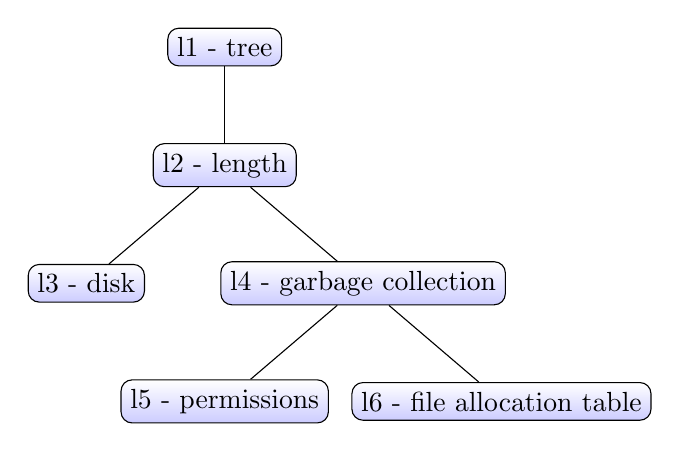
\begin{tikzpicture}[sibling distance=10em,
      every node/.style = {shape=rectangle, rounded corners,
        draw, align=center,
        top color=white, bottom color=blue!20}]
    \node {l1 - tree}
    child { node {l2 - length}
      child { node {l3 - disk}}
      child { node {l4 - garbage collection}
        child { node {l5 - permissions}}
        child { node {l6 - file allocation table}}}};
  \end{tikzpicture}
\end{figure}

At this point in development, we have six models of the filesystem,
here referred to as \texttt{l1} through \texttt{l6} (see
table \ref{model-description-table}). Each new model
\textit{refines} a previous model, adding some features and
complexity, and thereby approaching closer to a model which is binary
compatible with FAT32. These refinement relationships are shown in
figure \ref{refinement-figure}. \texttt{l0} is the simplest of these,
representing the filesystem as a literal tree; later models feature
file metadata (including ownership and permissions), externalisation
of file contents, and allocation/file allocation using an allocation
vector after the fashion of the CP/M file system.

Broadly, we characterise the filesystem
operations we offer as either \textit{write} operations, which do
modify the filesystem, or \textit{read} operations, which do not. In
each model, we have been able to prove \textit{read-over-write}
properties which show that write operations have
their effects made available immediately for reads at the same
location, but also that they do not affect reads at other locations.

The first read-after-write theorem states that immediately following a
write of some text at some location, a read of the same length at the
same location yields the same text. The second read-after-write
theorem states that after a write of some text at some location, a
read at any other location returns exactly what it would have returned
before the write. As an example, listings for the \texttt{l1} versions
of these theorems follow.

\medskip

\noindent
\begin{verbatim}
(defthm l1-read-after-write-1
  (implies (and (l1-fs-p fs)
                (stringp text)
                (symbol-listp hns)
                (natp start)
                (equal n (length text))
                (stringp (l1-stat hns fs)))
           (equal (l1-rdchs hns (l1-wrchs hns fs start text) start n) text)))

(defthm l1-read-after-write-2
  (implies (and (l1-fs-p fs)
                (stringp text2)
                (symbol-listp hns1)
                (symbol-listp hns2)
                (not (equal hns1 hns2))
                (natp start1)
                (natp start2)
                (natp n1)
                (stringp (l1-stat hns1 fs)))
           (equal (l1-rdchs hns1 (l1-wrchs hns2 fs start2 text2) start1 n1)
                  (l1-rdchs hns1 fs start1 n1))))
\end{verbatim}

By composing these properties, we can reason about executions
involving multiple reads and writes, as shown in the following
throwaway lemma.

\medskip

\noindent
\begin{verbatim}
(thm
 (implies (and (l1-fs-p fs)
               (stringp text1)
               (stringp text2)
               (symbol-listp hns1)
               (symbol-listp hns2)
               (not (equal hns1 hns2))
               (natp start1)
               (natp start2)
               (stringp (l1-stat hns1 fs))
               (equal n1 (length text1)))
          (equal (l1-rdchs hns1
                           (l1-wrchs hns2 (l1-wrchs hns1 fs start1 text1)
                                     start2 text2)
                           start1 n1)
                 (l1-rdchs hns1 (l1-wrchs hns1 fs start1 text1)
                           start1 n1))))
\end{verbatim}

\section{Proof methodology}

In \textit{l1}, our simplest model, the read-over-write properties
were, of necessity, proven from scratch, with the use of some rather
complicated induction schemes. For reference, the following code listing shows
the induction scheme used for \texttt{l1-read-after-write-2}.

\medskip

\noindent
\begin{verbatim}
(defun induction-scheme (hns1 hns2 fs)
  (if (atom hns1)
      fs
    (if (atom fs)
        nil
      (let ((sd (assoc (car hns2) fs)))
        (if (atom sd)
            fs
          (if (atom hns2)
              fs
            (if (not (equal (car hns1) (car hns2)))
                fs
              (let ((contents (cdr sd)))
                (if (atom (cdr hns1))
                    (cons (cons (car sd)
                                contents)
                          (delete-assoc (car hns2) fs))
                  (cons (cons (car sd)
                              (induction-scheme (cdr hns1) (cdr hns2) contents))
                                (delete-assoc (car hns2) fs)))))))))))
\end{verbatim}

In each subsequent model, the read-over-write properties are proven as
corollaries of equivalence proofs which establish the correctness of
read and write operations in the respective model with respect to a
previous model. A representation of such an equivalence proof can be
seen in figures \ref{l2-wrchs-correctness-1},
\ref{l2-rdchs-correctness-1} and \ref{l2-read-over-write-1}, which
respectively show the equivalence proof for \texttt{l2-wrchs}, the
equivalence proof for \texttt{l2-rdchs} and the composition of these
to obtain the first read-over-write theorem for model \texttt{l2}.


\begin{figure}
  \centering
  \caption{l2-wrchs-correctness-1}
  \label{l2-wrchs-correctness-1}
  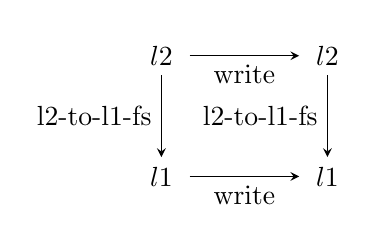
\begin{tikzpicture}
    \matrix (m) [matrix of math nodes,row sep=3em,column sep=4em,minimum width=2em]
            {
              l2 & l2 \\
              l1 & l1 \\};
            \path[-stealth]
            (m-1-1) edge node [left] {l2-to-l1-fs} (m-2-1)
            edge node [below] {write} (m-1-2)
            (m-2-1.east|-m-2-2) edge node [below] {write} (m-2-2)
            (m-1-2) edge node [left] {l2-to-l1-fs} (m-2-2);
  \end{tikzpicture}
\end{figure}

\begin{figure}
  \centering
  \caption{l2-rdchs-correctness-1}
  \label{l2-rdchs-correctness-1}
  \begin{tikzpicture}
    \matrix (m) [matrix of math nodes,row sep=3em,column sep=4em,minimum width=2em]
            {
              l2 & text \\
              l1 \\};
            \path[-stealth]
            (m-1-1) edge node [left] {l2-to-l1-fs} (m-2-1)
            edge node [below] {read} (m-1-2)
            (m-2-1.east|-m-2-2) edge node [below] {read} (m-1-2);
  \end{tikzpicture}
\end{figure}

\begin{figure}
  \centering
  \caption{l2-read-over-write-1}
  \label{l2-read-over-write-1}
  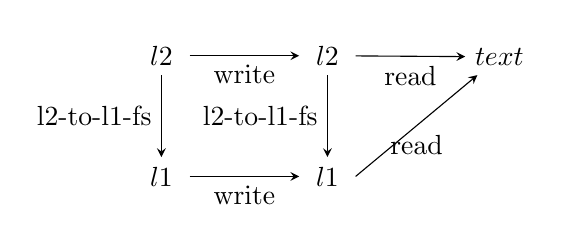
\begin{tikzpicture}
    \matrix (m) [matrix of math nodes,row sep=3em,column sep=4em,minimum width=2em]
            {
              l2 & l2 & text \\
              l1 & l1 \\};
            \path[-stealth]
            (m-1-1) edge node [left] {l2-to-l1-fs} (m-2-1)
            edge node [below] {write} (m-1-2)
            (m-2-1.east|-m-2-2) edge node [below] {write} (m-2-2)
            (m-1-2) edge node [left] {l2-to-l1-fs} (m-2-2)
            edge node [below] {read} (m-1-3)
            (m-2-2.east) edge node [below] {read} (m-1-3);
  \end{tikzpicture}
\end{figure}

\section{Some proof details}

\subsection{Invariants}

As the models grow more complex, with the addition of more auxiliary
data the "sanity" criteria for filesystem instances become more
complex. For instance, in \texttt{l4}, the predicate \texttt{l4-fs-p}
is defined to be the same as \texttt{l3-fs-p}, which recursively
defines the shape of a valid filesystem. However, a "sane" filesystem
requires also that each disk index assigned to a regular file be
marked as \textit{used} in the allocation vector, and that it be
distinct from other disk indices assigned to files across the
filesystem. These properties are invariants to be maintained across
write operations; they simplify the verification of read-after-write
properties by ensuring that write properties do not create an
"aliasing" situation in which a regular file's contents can be
modified through a write to a different regular file.

These properties, in the form of the predicates
\texttt{indices-marked-listp} and \texttt{no-duplicatesp}, are
packaged together into the \texttt{l4-stricter-fs-p} predicate, for
which a listing follows.

\medskip

\noindent
\begin{verbatim}
(defun l4-stricter-fs-p (fs alv)
  (declare (xargs :guard t))
  (and (l4-fs-p fs)
       (boolean-listp alv)
       (let ((all-indices (l4-list-all-indices fs)))
            (and (no-duplicatesp all-indices)
                 (indices-marked-p all-indices alv)))))
\end{verbatim}

\subsection{Performance hacking}

As in all ACL2 verification efforts, our work accumulated a number of
helper functions and lemmata in the service of the big-picture proofs,
and these were prone to slow down our proofs somewhat. Thus, using
ACL2's \texttt{accumulated-persistence} tool, we made an effort to
trim the number of enabled rules by focussing on the rules which the
tool suggested to be \textit{useless}. This was important in helping us reduce
the certification time for \texttt{l6} from 229 seconds to 84 seconds,
but from this point onwards results were mixed. As an illustrative
example, disabling the function \texttt{l6-wrchs} brought down the
certification time for \textt{l6} from 84 seconds to 60 seconds, yet
disabling another function, \texttt{l4-collect-all-index-lists}, had a
negligible effect on other books and actually served to increase the
certification time from 60 seconds to 69 seconds. Needless to say, the
latter change was rolled back; a pertinent explanation can be found in
the ACL2 documentation topic \texttt{accumulated-persistence-subtleties}.

%%  It is interesting to note that disabling
%%  l4-collect-all-index-lists brings down the certification time for l4
%%  from 19 seconds to 18 seconds, the certification time for l5 from
%%  21 seconds to 22 seconds and the
%% that for l6 from 60 seconds to 69 seconds.
%% It is interesting to note that disabling l6-wrchs brings down the
%% certification time for \texttt{l6} from 84 seconds to 60 seconds.

\section{Evaluation}
At present, the codebase spans 11710 lines of ACL2 code, including 152
function definitions and 616 theorems and lemmas. Some of this data was
obtained by David A. Wheeler's sloccount tool.

In table \ref{certification-timing-table} we note the time taken to certify
the models in ACL2, as well as some infrastructure upon which the
models are built.

\begin{table}[]
  \centering
  \caption{Time take to prove models}
  \label{certification-timing-table}
  \begin{tabular}{ll}
    \texttt{l1} & 1s \\
    \texttt{l2} & 5s \\
    \texttt{l3} & 6s \\
    \texttt{l4} & 19s \\
    \texttt{l5} & 21s \\
    \texttt{l6} & 60s \\
    Misc. & 4s \\
  \end{tabular}
\end{table}

\section{Future work}

We are pursuing future work in a few different directions.

\subsection{FAT32}

Having modelled the file allocation table, the next step is to
dispense with the tree representation and implement filesystem
traversal by looking up entries in directory files. This will yield a
model which is entirely contained in a disk data structure and which
can further be validated by co-simulation with a FAT32 implementation,
such as the one shipped with the Linux kernel.

\subsection{Other filesystems}

We plan to model a filesystem with journalling in order to prove crash
consistency; we are considering ext4 and NTFS. We may also incorporate
reasoning about non-determinism in multiprogramming environments where
the filesystem is accessed by multiple processes concurrently.

\subsection{fsck}
Another goal of this work is to provide a basis for reasoning about
\texttt{fsck} and other tools for sanity checking and recovering data
from a filesystem. This is a large part of the motivation for pursuing
binary compatibility.

\subsubsection*{Acknowledgments.} This work has been supported by a
grant from the NSF.

\section{References}\label{references}

\bibliographystyle{splncs}
\bibliography{references}

\end{document}
